\subsection{Glyph: \glyph{Unspecified activity}}
\label{af:sec:unspecifiedActivity}

The simplest type of AN is the \glyph{unspecified activity}: one whose type is unknown or simply not relevant to the purposes of the model.  This arises, for example, when the nature of the activity is unknown, either to a known entity or an entity that has been inferred indirectly, or when the entity is merely a construct introduced for the needs of the model, without direct biological relevance.

\begin{glyphDescription}

\glyphSboTerm SBO:

\glyphContainer An \glyph{unspecified activity} is represented by an elliptic container, as shown in \fig{af:unspecified}.

\glyphLabel An \glyph{unspecified actifity} is identified by a label placed in an unbordered box containing a string of characters.  The characters can be distributed on several lines to improve readability, although this is not mandatory.  The label box must be attached to the center of the container.  The label may spill outside of the container.

\end{glyphDescription}

\begin{figure}[H]
  \centering
  \includegraphics[scale = 0.3]{images/unspecified}
  \caption{The \AF glyph for \glyph{unspecified activity}.}
  \label{fig:af:unspecified}
\end{figure}



% The following is for [X]Emacs users.   Please leave in place.
% Local Variables:
% TeX-master: "../sbgn_PD-level1"
% End:
